\documentclass[10pt]{article}

\usepackage[margin=0.75in]{geometry}
\usepackage{amsmath,amsthm,amssymb}
\usepackage{xcolor}
\usepackage{cancel}
\usepackage{graphicx}
\usepackage{changepage}
\usepackage{circuitikz}
\usepackage{pgfplots}
\usepackage{physics}
\usepackage{hyperref}
\usepackage{siunitx}
\usepackage{fontspec}
\usepackage{relsize}
\usepackage{subfig}
\usepackage{todonotes}
\usepackage{minted}
\usepackage{multicol, multirow, booktabs}
\usepackage[breakable]{tcolorbox}
\usepackage[inline]{enumitem}

\theoremstyle{definition}
\newtheorem{problem}{Problem}
\newtheorem{soln}{Solution}

\pgfplotsset{compat=newest}
\usetikzlibrary{lindenmayersystems}
\usetikzlibrary{arrows}
\usetikzlibrary{calc}
\usetikzlibrary{positioning, fit}
\usetikzlibrary{3d, perspective}

\definecolor{incolor}{HTML}{303F9F}
\definecolor{outcolor}{HTML}{D84315}
\definecolor{cellborder}{HTML}{CFCFCF}
\definecolor{cellbackground}{HTML}{F7F7F7}
\newcommand{\ui}{\hat{i}}
\newcommand{\uj}{\hat{j}}
\newcommand{\uk}{\hat{k}}
\newcommand{\ux}{\hat{x}}
\newcommand{\uy}{\hat{y}}
\newcommand{\uz}{\hat{z}}
\newcommand{\primed}[1]{#1^\prime}
\pgfdeclarelayer{background}  
\pgfsetlayers{background,main}
\AtBeginDocument{\RenewCommandCopy\qty\SI}

\makeatletter
\newcommand{\boxspacing}{\kern\kvtcb@left@rule\kern\kvtcb@boxsep}
\makeatother
\newcommand{\prompt}[4]{
    \ttfamily\llap{{\color{#2}[#3]:\hspace{3pt}#4}}\vspace{-\baselineskip}
}

\newcommand{\thevenin}[2]{
  \begin{center}
    \begin{circuitikz} \draw
      (0,0) -- (2,0) to[battery1, l_=$V_{Th}\eq#1$] (2,2) 
      to[resistor, l_=$R_{Th}\eq#2$] (0,2)
      ;
      \draw [o-] (-.07,2.079);
      \draw [o-] (-.07,0.079);
    \end{circuitikz}
  \end{center}
}

\newcommand{\norton}[2]{
  \begin{center}
    \begin{circuitikz} \draw
      (0,0) -- (3,0) to[american current source, l_=$I_{N}\eq#1$] (3,2) -- (0,2) (2,0)
      to[resistor, l=$R_{N}\eq#2$] (2,2)
      ;
      \draw [o-] (-.07,2.079);
      \draw [o-] (-.07,0.079);
    \end{circuitikz}
  \end{center}
}

\newcommand{\highlight}[1]{\colorbox{yellow}{$\displaystyle #1$}}

\newcommand{\ti}[1]{\widetilde{#1}}

\newfontface{\Kaufmann}{Kaufmann}
\DeclareTextFontCommand{\kf}{\Kaufmann}
\newcommand{\scriptr}{\fontsize{12pt}{12pt}\kf{r}}

\newfontface{\KaufmannB}{Kaufmann Bd BT}
\DeclareTextFontCommand{\kfb}{\KaufmannB}
\newcommand{\bscriptr}{\fontsize{12pt}{12pt}\kfb{r}}

\newcommand{\bv}[1]{\mathbf{#1}}

\title{Physics 3610H: Assignment IV}
\author{Jeremy Favro (0805980) \\ Trent University, Peterborough, ON, Canada}
\date{\today}

\begin{document}
\maketitle

% PROBLEM 1
\begin{problem}
Consider the following one-dimensional potential:
$$
  V(x)=\begin{cases}
    0   & x<0 \\
    V_0 & x>0
  \end{cases}
$$
Determine the \colorbox{yellow}{transmission coefficient} (assuming this is actually supposed to be reflection)
$R$ for a wave of energy $E > V_0 > 0$ incident from the
left, following these steps:
The solutions to the time-independent Schrodinger equation have the following form in the
two regions:
\begin{table}[h]
  \centering
  \begin{tabular}{c|c}
    $x<0$                        & $x>0$                        \\
    \hline
    $e^{+ikx}$ and/or $e^{-ikx}$ & $e^{+iqx}$ and/or $e^{-iqx}$
  \end{tabular}
\end{table}
\begin{enumerate}[label=(\alph*)]
  \item Write expressions for $k$ and $q$ in terms of $E$ and $V_0$.
  \item Consider a wave incident from the left. Write expressions for the wavefunction in the
        two regions. For $x < 0$, there are two terms, both an incident wave and a reflected wave,
        while for $x > 0$ there is only one, the transmitted wave. Use the coefficient $A$ for the incident
        wave, $B$ for the reflected wave, and $C$ for the transmitted wave.
  \item List all the conditions which the full wavefunction must satisfy
  \item Is the energy quantized?
  \item Apply the conditions in (c) to determine the reflection coefficient $R$. Recall that $R$ is the
        ratio of the reflected probability current density to the incident probability current density.
        In the notation established here that means $R = |B|^2/|A|^2$. Note that you do not need to
        determine each coefficient, only this ratio. Your answer should be expressed in terms of $E$
        and $V_0$.
\end{enumerate}
\end{problem}
\begin{soln}
  \begin{enumerate}[label=(\alph*)]
    \item As usual
          $$k=\sqrt{\frac{2mE}{\hbar^2}}$$
          because the particle has relative energy $E$ in the region where $V(x)=0$.
          For the $V(x)=V_0$ region the particle has relative energy $E-V_0$ as we've
          been told $E>V_0$ so
          $$q=\sqrt{\frac{2m(E-V_0)}{\hbar^2}}$$
    \item We have
          $$\psi(x)=\begin{cases}
              Ae^{ikx}+Be^{-ikx} & x<0 \\
              Ce^{iqx}           & x>0
            \end{cases}
          $$
          because the positive exponents (when coupled with the time part) give a wave moving to the right and the negatives
          one moving to the left. Because the transmitted wave is moving exclusively to the left we use only the positive exponential.
    \item The full wavefunction must be continuous, smooth, and normalized (though this isn't a normalizable state?).
          In our case because our functions are obviously smooth and continuous by nature of being exponentials the only place
          we need to worry about smoothness and continuity is at the interface $x=0$. Using the definitions of smoothness and continuity we get then that
          \begin{align*}
            \psi(0^-)=\psi(0^+)\implies A+B=C                                               \\
            \eval{\frac{d\psi}{dx}}_{0^-}=\eval{\frac{d\psi}{dx}}_{0^+}\implies Aik-Bik=Ciq \\
          \end{align*}
    \item No, because there is no restriction imposed by the above conditions that would imply (or rather, require) quantization.
    \item Starting with our second condition,
          $$Aik-Bik=Ciq\implies A-B=C\frac{q}{k}.$$
          Then using our first condition,
          \begin{align*}
                     & A-B=(A+B)\frac{q}{k}                                                                                                                    \\
            \implies & A-A\frac{q}{k}=B+B\frac{q}{k}                                                                                                           \\
            \implies & A\left(1-\frac{q}{k}\right)=B\left(1+\frac{q}{k}\right)                                                                                 \\
            \implies & \abs{B}^2/\abs{A}^2=\abs{B/A}^2=\abs{\frac{1-\frac{q}{k}}{1+\frac{q}{k}}}^2=\abs{\frac{k-q}{k+q}}^2                                     \\
            \implies & \abs{\frac{\sqrt{\frac{2mE}{\hbar^2}}-\sqrt{\frac{2m(E-V_0)}{\hbar^2}}}{\sqrt{\frac{2mE}{\hbar^2}}+\sqrt{\frac{2m(E-V_0)}{\hbar^2}}}}^2 \\
            \implies & \abs{\frac{\sqrt{E}-\sqrt{E-V_0}}{\sqrt{E}+\sqrt{E-V_0}}}^2
          \end{align*}
  \end{enumerate}
\end{soln}

% PROBLEM 2
\begin{problem}
Consider a system consisting of five beads equally spaced along a massless, elastic string.
\begin{center}
  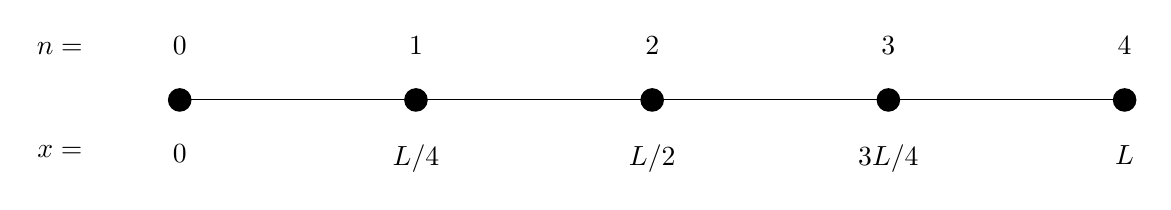
\begin{tikzpicture}
    \def\radius{0.15}
    \def\ulen{3}
    \draw (0,0) -- (4*\ulen,0);
    \fill (0,0) circle (\radius)
    node[below=0.15*\ulen]{$0$}
    node[above=0.15*\ulen]{$0$}
    node[above=0.15*\ulen]{$n=\qquad~~~~~~~~~~~~~~~~~~~~$}
    node[below=0.15*\ulen]{$x=\qquad~~~~~~~~~~~~~~~~~~~~$};
    \fill (1*\ulen,0) circle (\radius) node[below=0.15*\ulen]{$L/4$} node[above=0.15*\ulen]{$1$};
    \fill (2*\ulen,0) circle (\radius) node[below=0.15*\ulen]{$L/2$} node[above=0.15*\ulen]{$2$};
    \fill (3*\ulen,0) circle (\radius) node[below=0.15*\ulen]{$3L/4$} node[above=0.15*\ulen]{$3$};
    \fill (4*\ulen,0) circle (\radius) node[below=0.15*\ulen]{$L$} node[above=0.15*\ulen]{$4$};
  \end{tikzpicture}
\end{center}
The beads on each end are held fixed. The three beads in the middle can move up and down
(but not along the string or in or out of the page). This system has only three degrees of
freedom: the up and down motion of each of the three central beads. The following three
functions form a complete set, in terms of which any allowed displacement of these beads
can be expressed.
$$
  g_1(x)=\frac{1}{\sqrt{2}}\sin\frac{\pi x}{L};
  \qquad g_2(x)=\frac{1}{\sqrt{2}}\sin\frac{2\pi x}{L};
  \qquad g_3(x)=\frac{1}{\sqrt{2}}\sin\frac{3\pi x}{L}
$$
Note that we consider in this problem only the positions of the beads and not the string.
The $x$ values in this problem are therefore discrete: $x_n = nL/4$ with $n = 1, 2, 3$.
\begin{enumerate}[label=(\alph*)]
  \item Show that $g_1(x)$ is normalized
  \item Show that $g_1(x)$ and $g_2(x)$ are orthogonal
  \item Consider a triangle wave, such as you might get from plucking the string in the middle.
        $$f(x_1)=L/4;\qquad f(x_2)=L/2;\qquad f(x_3)=L/4.$$
        Determine the values of $a_k$ such that
        $$f(x)=\sum_k a_kg_k(x).$$
  \item Check your result by plotting the positions of the bead generated by this sum.
\end{enumerate}
\end{problem}
\begin{soln}~
  \begin{enumerate}[label=(\alph*)]
    \item For normalization we require that the self-inner product be 1,
          $$\sum_{n=1}^{3}g_1(x_n)g_1(x_n)=\sum_{n=1}^{3}g_1^2(x_n)=1.$$
          Evaluating this we get
          \begin{align*}
             & =\sum_{n=1}^{3}g_1^2(x_n)                                                                         \\
             & =\frac{1}{2}\left[\sin^2\frac{\pi x_1}{L}+\sin^2\frac{\pi x_2}{L}+\sin^2\frac{\pi x_3}{L}\right]  \\
             & =\frac{1}{2}\left[\sin^2\frac{\pi L/4}{L}+\sin^2\frac{\pi L/2}{L}+\sin^2\frac{\pi 3L/4}{L}\right] \\
             & =\frac{1}{2}\left[\sin^2\frac{\pi}{4}+\sin^2\frac{\pi}{2}+\sin^2\frac{3\pi}{4}\right]             \\
             & =\frac{1}{2}\left[\frac{1}{2}+1+\frac{1}{2}\right]=1
          \end{align*}
    \item For orthogonality we require that the inner product of $g_1$ and $g_2$ be zero,
          \begin{align*}
             & =\sum_{n=1}^{3}g_1(x_n)g_2(x_n)                               \\
             & =\frac{1}{2}\left[\sin\frac{\pi x_1}{L}\sin\frac{2\pi x_1}{L}
              +\sin\frac{\pi x_2}{L}\sin\frac{2\pi x_2}{L}
              +\sin\frac{\pi x_3}{L}\sin\frac{2\pi x_3}{L}
            \right]                                                          \\
             & =\frac{1}{2}\left[\sin\frac{\pi L/4}{L}\sin\frac{2\pi L/4}{L}
              +\sin\frac{\pi L/2}{L}\sin\frac{2\pi L/2}{L}
              +\sin\frac{\pi 3L/4}{L}\sin\frac{2\pi 3L/4}{L}
            \right]                                                          \\
             & =\frac{1}{2}\left[\sin\frac{\pi}{4}\sin\frac{\pi}{2}
              +\sin\frac{\pi}{2}\sin\pi
              +\sin\frac{3\pi}{4}\sin\frac{3\pi}{2}
            \right]                                                          \\
             & =\frac{1}{2}\left[\frac{1}{\sqrt{2}}
              +0
              -\frac{1}{\sqrt{2}}
              \right]=0
          \end{align*}
    \item This wave looks like
          \begin{center}
            \begin{tikzpicture}
              \def\radius{0.15}
              \def\ulen{3}
              \fill (0,0) coordinate(zero) circle (\radius)
              node[below=0.15*\ulen]{$0$}
              node[above=0.15*\ulen]{$0$};
              \fill (1*\ulen,0.25*\ulen) coordinate(one) circle (\radius)
              node[above=0.15*\ulen]{$1$};
              \fill (2*\ulen,0.5*\ulen) coordinate(two) circle (\radius)
              node[above=0.15*\ulen]{$2$};
              \fill (3*\ulen,0.25*\ulen) coordinate(three) circle (\radius)
              node[above=0.15*\ulen]{$3$};
              \fill (4*\ulen,0) coordinate(four) circle (\radius)
              node[below=0.15*\ulen]{$L$}
              node[above=0.15*\ulen]{$4$};


              \draw (zero)--(one)--(two)--(three)--(four);
              \draw[dashed] (zero)--(four);
            \end{tikzpicture}
          \end{center}
          Generally we are looking to write
          $$f(x)=\frac{1}{\sqrt{2}}\left[a_1\sin\frac{\pi x}{L}
              +a_2\sin\frac{2\pi x}{L}+a_3\sin\frac{3\pi x}{L}
              \right]$$
          which gives three equations to use to determine $a_{1,2,3}$:
          \begin{align}
            f(L/4)  & =\frac{1}{\sqrt{2}}\left[\frac{a_1}{\sqrt{2}}+a_2+\frac{a_3}{\sqrt{2}}\right]=L/4 \\
            f(L/2)  & =\frac{1}{\sqrt{2}}\left[a_1-a_3\right]=L/2                                       \\
            f(3L/4) & =\frac{1}{\sqrt{2}}\left[\frac{a_1}{\sqrt{2}}-a_2+\frac{a_3}{\sqrt{2}}\right]=L/4 \\
          \end{align}
          Setting (1) and (3) equal,
          \begin{align*}
            \frac{1}{\sqrt{2}}\left[\frac{a_1}{\sqrt{2}}+a_2+\frac{a_3}{\sqrt{2}}\right] & =\frac{1}{\sqrt{2}}\left[\frac{a_1}{\sqrt{2}}-a_2+\frac{a_3}{\sqrt{2}}\right] \\
            \implies  \frac{a_1}{\sqrt{2}}+a_2+\frac{a_3}{\sqrt{2}}                      & =\frac{a_1}{\sqrt{2}}-a_2+\frac{a_3}{\sqrt{2}}                                \\
            \implies  a_2                                                                & =-a_2\implies a_2=0
          \end{align*}
          Then solving (2) for $a_1$,
          \begin{align*}
            \frac{1}{\sqrt{2}}\left[a_1-a_3\right] & =L/2             \\
            \implies  a_1                          & =L\sqrt{2}/2+a_3
          \end{align*}
          Which, using (1), gets us
          \begin{align*}
            \frac{a_1}{\sqrt{2}}+\frac{a_3}{\sqrt{2}} & =L\sqrt{2}/4                            \\
            \implies a_1+a_3                          & =L/2                                    \\
            \implies L\sqrt{2}/2+a_3 +a_3             & =L/2                                    \\
            \implies a_3                              & =L/4-L\sqrt{2}/4=\frac{1+\sqrt{2}}{4}L.
          \end{align*}
          Which gives
          $$a_1=L\sqrt{2}/2+a_3=L\sqrt{2}/2+L/4-L\sqrt{2}/4=\frac{1-\sqrt{2}}{4}L.$$
          We could probably have come up with these using some kind of variation on Fourier's trick but this method was what first
          popped in to my head.
    \item We've written
          $$f(x)=\frac{1}{\sqrt{2}}\left[\frac{1+\sqrt{2}}{4}L\sin\frac{\pi x}{L}
              +\frac{1-\sqrt{2}}{4}L\sin\frac{3\pi x}{L}
              \right]=\frac{\left(\sqrt{2} - 2\right) L \sin\left(\frac{3\pi x}{L}\right)+\left(\sqrt{2} + 2\right) L \sin\left(\frac{\pi x}{L}\right)}{8}.$$
          Which gives the following plot where green circles represent $f(x)$ and black dots represent the expected positions by the definition of $f(x)$,
          \begin{center}
            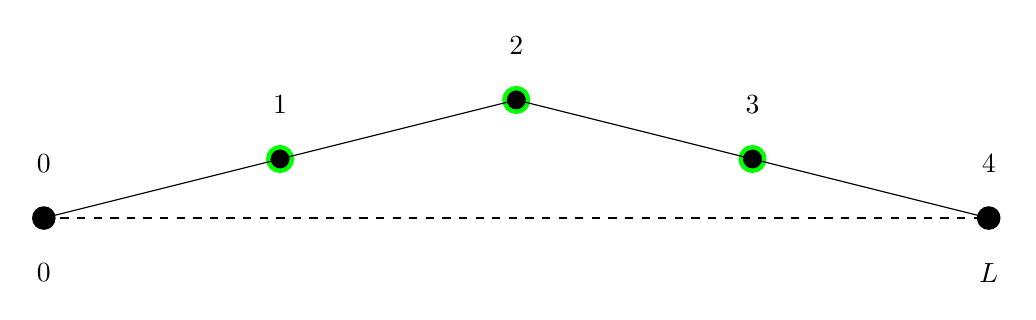
\begin{tikzpicture}
              \def\radius{0.15}
              \def\ulen{3}
              \fill (0,0) coordinate(zero) circle (\radius)
              node[below=0.15*\ulen]{$0$}
              node[above=0.15*\ulen]{$0$};

              \fill (1*\ulen,0.25*\ulen) coordinate(one) circle (\radius)
              node[above=0.15*\ulen]{$1$};
              \def\x{\ulen/4}
              \draw[green,ultra thick,trig format=rad] (1*\ulen,
              {((sqrt(2) - 2) * \ulen * sin((3 * pi * \x) / \ulen)) / 8 + ((sqrt(2) + 2) * \ulen * sin((pi * \x) / \ulen)) / 8}) circle (\radius);

              \fill (2*\ulen,0.5*\ulen) coordinate(two) circle (\radius)
              node[above=0.15*\ulen]{$2$};
              \def\x{2*\ulen/4}
              \draw[green,ultra thick,trig format=rad] (2*\ulen,
              {((sqrt(2) - 2) * \ulen * sin((3 * pi * \x) / \ulen)) / 8 + ((sqrt(2) + 2) * \ulen * sin((pi * \x) / \ulen)) / 8}) circle (\radius);

              \fill (3*\ulen,0.25*\ulen) coordinate(three) circle (\radius)
              node[above=0.15*\ulen]{$3$};
              \def\x{3*\ulen/4}
              \draw[green,ultra thick,trig format=rad] (3*\ulen,
              {((sqrt(2) - 2) * \ulen * sin((3 * pi * \x) / \ulen)) / 8 + ((sqrt(2) + 2) * \ulen * sin((pi * \x) / \ulen)) / 8}) circle (\radius);

              \fill (4*\ulen,0) coordinate(four) circle (\radius)
              node[below=0.15*\ulen]{$L$}
              node[above=0.15*\ulen]{$4$};


              \draw (zero)--(one)--(two)--(three)--(four);
              \draw[dashed] (zero)--(four);
            \end{tikzpicture}
          \end{center}
          (Generated with TikZ)
  \end{enumerate}
\end{soln}
\end{document}